% =============================================================================
%
% This is the LaTeX source code of the lecture notes.
%
%
% Author:   Blazej Bucha
% Year:     2022
% Contact:  blazej.bucha@stuba.sk
% Encoding: UTF-8
%
% =============================================================================






% LaTeX Packages
% =============================================================================

\documentclass[a4paper, 12pt]{book}
\usepackage[slovak]{babel}
\usepackage[utf8]{inputenc}
\usepackage[round]{natbib}
\usepackage{amsmath}
\usepackage{upgreek}
\usepackage{listings}
\usepackage{xcolor}
\usepackage{graphicx}
\usepackage{accsupp}
\usepackage[unicode,
            pdfborder={0 0 0},
            colorlinks=true,
            urlcolor=blue,
            citecolor=blue,
            linkcolor=blue]{hyperref}
\usepackage[top=2.5cm, bottom=2.5cm, left=2.5cm, right=2.5cm]{geometry}
\linespread{1.2}

% =============================================================================






% Define and set the style of code listings
% =============================================================================

% Define custom colours
\definecolor{comments}{rgb}{0.65, 0.65, 0.65}
\definecolor{strings}{rgb}{0.0, 0.3, 0.7}
\definecolor{linenumbers}{rgb}{0.5, 0.5, 0.5}
\definecolor{keywords}{rgb}{0.85, 0.0, 0.0}
\definecolor{backcolour}{rgb}{0.98, 0.98, 0.98}


% Define custom listing style
\lstdefinestyle{codestyle}
{
    backgroundcolor=\color{backcolour},
    commentstyle=\color{comments},
    keywordstyle=\color{keywords},
    numberstyle=\tiny\noncopynumber,
    columns=flexible,
    stringstyle=\color{strings},
    basicstyle=\ttfamily\footnotesize,
    breakatwhitespace=false,
    breaklines=true,
    captionpos=b,
    keepspaces=true,
    numbers=left,
    numbersep=5pt,
    showspaces=false,
    showstringspaces=false,
    showtabs=false,
    tabsize=2
}


% Defines a new command that ensures we can copy the source code from the 
% compiled PDF without copying the line numbers
\newcommand{\noncopynumber}[1]
{
    \BeginAccSupp{method=escape,ActualText={}}
    #1
    \EndAccSupp{}
}


% Apply the custom listing style
\lstset{style=codestyle}


% It seems the "listings" package is not able to encode the nice special Slovak 
% characters such as "á", "ľ", etc.  Next follows a brute force solution.
\lstset{
  literate={á}{{\'a}}1
           {ä}{{\" a}}1
           {č}{{\v c}}1
           {ď}{{d\kern-0.07cm\char39\kern-0.07cm}}1
           {é}{{\'e}}1
           {í}{{\'i}}1
           {ĺ}{{\'l}}1
           {ľ}{{l\kern-0.12cm\char39\kern-0.05cm}}1
           {ň}{{\v n}}1
           {ó}{{\'o}}1
           {ô}{{\^o}}1
           {ŕ}{{\'r}}1
           {š}{{\v s}}1
           {ť}{{t\kern-0.10cm\char39\kern-0.05cm}}1
           {ú}{{\'u}}1
           {ý}{{\'y}}1
           {ž}{{\v z}}1
           {Á}{{\'A}}1
           {Ä}{{\" A}}1
           {Č}{{\v C}}1
           {Ď}{{\v D}}1
           {É}{{\'E}}1
           {Í}{{\'I}}1
           {Ĺ}{{\'L}}1
           {Ľ}{{L\kern-0.12cm\char39\kern-0.00cm}}1
           {Ň}{{\v N}}1
           {Ó}{{\'O}}1
           {Ô}{{\^O}}1
           {Ŕ}{{\'R}}1
           {Š}{{\v S}}1
           {Ť}{{\v T}}1
           {Ú}{{\'U}}1
           {Ý}{{\'Y}}1
           {Ž}{{\v Z}}1
}


% Add the "as" keyword to the Python listings
\lstdefinelanguage{mypython}[]{Python}{morekeywords={as,True,False}}


% Caption title for listings
\renewcommand\lstlistingname{Zdrojový kód}

% =============================================================================






% Custom commands
% =============================================================================
\newcommand{\diff}{\mathrm d}
\newcommand{\grad}{\mathrm{grad}}
\newcommand{\gidx}{\mathrm g}
\newcommand{\cidx}{\mathrm c}
\let\vec\mathbf

% Let's change the "Dodatok" label of chapters after Conclusions to "Príloha"
\addto\captionsslovak{\renewcommand\appendixname{Príloha}}

% =============================================================================






% =============================================================================

\sloppy
\begin{document}

% -----------------------------------------------------------------------------
\tableofcontents
\newpage
% -----------------------------------------------------------------------------






% -----------------------------------------------------------------------------

\chapter*{Predslov}

Mnohé geodetické merania a úkony využívajú pôsobenie tiažového poľa alebo sú 
ním ovplyvnené, od použitia olovnice až po merania založené na globálnych 
navigačných družicových systémoch.  Táto práca sa zaoberá tiažovým poľom 
s dôrazom na geodetický kontext.  Určená je predovšetkým ako doplňujúci učebný 
text k predmetom \emph{Fyzikálna geodézia~1} a \emph{Fyzikálna geodézia~2} pre 
študentov odboru Geodézia a kartografia Stavebnej fakulty STU.  Niektoré časti 
by azda mohli byť užitočné pre širší okruh čitateľov, či už ide o študentov 
príbuzných vedných odborov alebo jednoducho o záujemcov o problematiku 
gravitačného a tiažového poľa.

Popísané sú základné princípy gravitačného a tiažového poľa vychádzajúce 
z Newtonovho gravitačného zákona 
(Kapitola~\ref{sec:gravitational_and_gravity_field}), sférické harmonické 
funkcie (Kapitola~\ref{sec:spherical_harmonics}), normálne a poruchové pole 
Zeme (Kapitoly~\ref{sec:normal_gravity_field} a \ref{sec:disturbing_field}) 
a základy určovania geoidu (Kapitola~\ref{sec:geoid_determination}).  Zvolili 
sme formu, ktorú na základe desaťročných skúseností s výučbou fyzikálnej 
geodézie považujeme za najvhodnejšiu pre očakávaných čitateľov, študentov 
geodézie a kartografie.  Znamená to, že hoci intelektuálne potešenie zo 
spoznávania tiažového poľa je bezodné, predsa len si vyžaduje pokročilé 
matematické zručnosti a nepochybne i isté zanietenie.  Snažili sme sa preto 
o výklad, ktorý by bol jednoduchý, zrozumiteľný, úplný, nápomocný a súčasne 
i podnecujúci.  Na miestach, kde sme to považovali za vhodné, doplnili sme text 
o počítačový kód prakticky demonštrujúci diskutovanú problematiku.  Spravidla 
ide o matematické koncepty, ktorých porozumenie si môže vyžadovať väčšie 
prvotné úsilie.  Nádejáme sa, že vlastným štúdiom, testovaním a úpravou tohto 
nenáročného kódu je možné jednoduchšie porozumieť diskutovanej problematike.

Bolo by prostoduché a azda i neskromné očakávať, že v práci sa nenájdu časti, 
ktoré mohli byť spracované zrozumiteľnejšie, či témy, ktoré v nej obsiahnuté 
nie sú, no mohli či mali byť diskutované.  Skôr ako za uzavretý študijný 
podklad považujeme tento učebný text za živý postupne sa zdokonaľujúci 
materiál.  Všetky zdrojové kódy sú preto voľne prístupné a pripomienkovateľné 
na adrese \url{https://github.com/blazej-bucha/physical-geodesy-lecture-notes}.

Práca bola napísaná v textovom editore Vim~v8.2 použitím typografického systému 
\TeX.  Skompilovaná bola programom \texttt{pdfTex}~v3.14159265-2.6-1.40.21.  
Mapy boli pripravené v \texttt{GMT}~v6.1.1.  Obrázky boli zhotovené v programe 
\texttt{Inkscape}~v1.0.2.  Väčšina uvedeného výpočtového kódu je napísaná 
a otestovaná v jazyku \texttt{Python}~v3.9.2 použitím modulov 
\texttt{NumPy}~v1.20.3, \texttt{Matplotlib}~v3.5.0 a \texttt{SciPy}~v1.7.3.  
Časť výpočtového kódu je napísaná v jazyku~C a v prostredí~MATLAB~R2021b.  
S týmito aplikáciami sme interagovali pod operačným systémom Debian GNU/Linux 
11 (Bullseye).  S výnimkou programu MATLAB ide o slobodný voľne šíriteľný 
software.  Vyslovujeme preto vďaku a slová ocenenia veľkej komunite 
excelentných programátorov za to, že poskytujú slobodný prvotriedny software.

Úprimné slová vďaky patria v neposlednom rade všetkým, ktorí akýmkoľvek 
spôsobom prispeli k tejto práci. \emph{Na záver tu budeš doplnený/á, ak s tým 
budeš súhlasiť!}


\vspace{4ex}

\noindent V Bratislave XX.~XX.~2022 \hfill Blažej Bucha




% -----------------------------------------------------------------------------

\chapter{Úvod}

Tvar Zeme možno definovať niekoľkými spôsobmi v závislosti od kontextu 
\citep{MoritzTheFigureOfTheEarth}.  Azda najprirodzenejšie je definovať tvar 
Zeme jej skutočným fyzickým povrchom, teda tou časťou Zeme, ktorá je viditeľná 
voľným okom.  Tento povrch obsahuje nespočetné množstvo zložitých terénnych 
útvarov, napríklad náhle ostré zmeny terénu.  Hoci sú takéto oblasti krásne na 
pohľad, znemožňujú aplikáciu istej časti potrebného matematického aparátu, 
napríklad plošnú integráciu.  Skúmať takto chápaný zemský povrch je preto možné 
iba po istom vyhladení.  Napriek vyhladeniu však ide o veľmi zložitú plochu.

K definovaniu tvaru Zeme môžeme pristúpiť i iným spôsobom.  Vieme, že približne 
dve tretiny zemského povrchu tvorí voda v podobe oceánov a morí.  Ak by sme 
s podobnou mierou hladkosti dokázali predĺžiť povrch oceánov a morí aj popod, 
resp. ponad pevnú časť zemského povrchu, získali by sme v porovnaní s fyzickým 
povrchom Zeme značne jednoduchší a hladší, no pritom stále verný tvar Zeme.  
Voda má za istých okolností navyše tú výhodnú vlastnosť, že existuje fyzikálna 
veličina, ktorá je na jej povrchu konštantná.  Táto vlastnosť by teda následne 
mohla umožniť akúsi predikciu morskej hladiny aj popod, resp. ponad kontinenty.  
Inými slovami, išlo by o geometricky jednoduchšiu plochu ako v predchádzajúcej 
definícii, navyše aj s istými relatívne jednoducho uchopiteľnými fyzikálnymi 
vlastnosťami.  Takáto definícia tvaru Zeme bola navrhnutá C. F. Gaussom 
(1777--1855) a podľa návrhu J. B. Listinga (1808--1882) nazývame túto plochu 
\emph{geoid}.  Veličina, ktorá je konštantná na povrchu geoidu sa nazýva 
\emph{tiažový potenciál}.

\emph{Fyzikálna geodézia} je vedná disciplína zaoberajúca sa určovaním tvaru 
Zeme, jej tiažovým poľom a ich zmenami v čase.  Študované sú oba vyššie opísané 
prístupy k tvaru Zeme, pričom historicky bol predmetom záujmu ako prvý geoid.  
Hoci prirodzená, no matematicky odvážna myšlienka určovať priamo fyzický povrch 
Zeme pochádza už od E. H. Brunsa (1848--1919), do popredia záujmu ju dostal až 
v polovici 20. storočia M. S. Molodenskij (1909--1991).  I v tomto prípade je 
však tvar Zeme určovaný z informácie o tiažovom poli.  Napĺňať jednu zo 
základných úloh geodézie, štúdium tvaru Zeme, teda znamená študovať aj tiažové 
pole Zeme.






% -----------------------------------------------------------------------------

\chapter{Gravitačné a tiažové pole}
\label{sec:gravitational_and_gravity_field}






\section{Newtonov gravitačný zákon}
\label{sec:newton_law}

Dva hmotné body $P$ a $Q$ nachádzajúce sa od seba vo vzdialenosti $l$ sa 
navzájom priťahujú \emph{gravitačnou silou}
%
\begin{equation}
\label{eq:newton_law}
\vec F_\gidx = -G \frac{m_P \, m_Q}{l^2} \, \frac{\vec r}{l}{.}
\end{equation}
%
Symbol $G$ označuje gravitačnú konštantu, $m_P$ a $m_Q$ predstavujú hmotnosti 
hmotných bodov a $\vec r$ je vektor definovaný bodmi $P$ a $Q$ so začiatkom 
v~bode $Q$.  Záporné znamienko v rovnici znamená, že vektor sily má začiatok 
v bode $P$ a smeruje do bodu $Q$ (Obrázok~\ref{fig:newton_law}).

\begin{figure}[b]
\centering
\input{./fig-newton-law.pdf_tex}
\caption{Gravitačná sila $\vec F_\gidx$, ktorou pôsobí hmotný bod $Q$ na hmotný 
bod $P$.  Vektor $\vec F_\gidx$ je z dôvodov vizualizácie mierne odsadený od 
spojnice bodov $P$ a $Q$}
\label{fig:newton_law}
\end{figure}

Rovnica~(\ref{eq:newton_law}) predstavuje \emph{gravitačný zákon} 
publikovaný I. Newtonom (1642--1727) v práci \emph{Philosophi\ae Naturalis 
Principia Mathematica} z roku 1687.  Hovorí, že každý hmotný bod vo vesmíre 
priťahuje každý iný hmotný bod silou, ktorej smer je daný spojnicou týchto 
bodov a veľkosť je priamo úmerná súčinu ich hmotností a nepriamo úmerná štvorcu 
ich vzdialenosti \citep{Kellogg1967}.  \emph{Hmotný bod} je idealizovaný pojem 
predstavujúci časticu s nulovým rozmerom a konečnou nenulovou hmotnosťou bez 
akýchkoľvek ďalších vlastností či štruktúry.  Hodnota gravitačnej konštanty 
odporúčaná od roku 2018 \emph{Komisiou pre dáta vo vede a technológiách} 
(CODATA) je
%
\begin{equation}
G = (6.67430 \pm 0.00015) \times 10^{-11} \ \mathrm{m}^3 \ \mathrm{kg}^{-1} 
\ \mathrm{s}^{-2}{.}
\end{equation}

Nech planéta obieha okolo Slnka (Obrázok~\ref{fig:orbital_motion}).  Označme 
polohu planéty v čase $t_0$ symbolom $P(t_0)$ a jej okamžitú rýchlosť symbolom 
$v(t_0)$.  Ak by Slnko prestalo pôsobiť na planétu gravitačnou silou, 
\emph{Newtonov pohybový zákon} hovorí, že planéta by sa ďalej pohybovala 
rovnomerným priamočiarym pohybom.  Za istý čas by sa teda dostala do bodu 
$P'(t_1)$.  Jediný spôsob ako zmeniť túto dráhu je pôsobením sily na planétu.  
Z rovnice~(\ref{eq:newton_law}) vyplýva, že v čase $t_0$ pôsobí na planétu 
gravitačnou silou $\vec F_\gidx(t_0)$ Slnko, pričom smer sily je daný spojnicou 
planéty a Slnka.  Gravitačná sila preto pritiahne planétu v smere vektora $\vec 
F_\gidx(t_0)$, čím zmení hypotetickú trajektóriu, ktorou by sa planéta 
pohybovala bez pôsobenia tejto sily.  V kombinácii s vektorom rýchlosti $\vec 
v(t_0)$ gravitačná sila spôsobí, že planéta sa dostane do bodu $P(t_1)$.  
V čase $t_1$ sa opísaná situácia opakuje, pričom vektory rýchlosti a sily už 
majú iný smer a s vysokou pravdepodobnosťou aj inú veľkosť.  Gravitačná sila 
Slnka teda zakrivuje trajektóriu planéty \emph{v každom okamihu}.
%
\begin{figure}
\centering
\input{./fig-orbital-motion.pdf_tex}
\caption{Obeh planéty okolo Slnka}
\label{fig:orbital_motion}
\end{figure}

Obdobným spôsobom je možné Newtonovým gravitačným zákonom vysvetliť i mnoho 
ďalších pozorovaných prírodných javov, napríklad príliv a odliv, či zodpovedať 
otázku, prečo majú planéty približne sférický tvar.  Je pozoruhodné, že hoci 
rovnica~(\ref{eq:newton_law}) bola odpozorovaná z pohybu nebeských telies, 
zhoduje sa i s experimentmi, ktoré boli vykonané na vzdialenosť niekoľkých 
desiatok mikrometrov \citep{Lee2020}.  Napriek uvedenému, azda je potrebné 
spomenúť i skutočnosť, že Newtonov gravitačný zákon je \emph{nesprávny} 
\citep{Feynman}.  Predpokladá napríklad, že zmena hmotnosti či vzdialenosti má 
okamžitý gravitačný účinok, teda i v prípade telies nachádzajúcich sa vo 
veľkých vzdialenostiach.  Tento predpoklad je však v rozpore s experimentálne 
potvrdenou Einsteinovou špeciálnou teóriou relativity.  Tá hovorí, že žiadny 
signál, a teda ani ten gravitačný, sa nemôže šíriť rýchlosťou väčšou ako je 
rýchlosť svetla.  Pre účely fyzikálnej geodézie sú však chyby spôsobené 
nepresnosťami Newtonovho gravitačného zákona väčšinou zanedbateľné, a tak táto 
teória, aj dnes, viac ako tristo rokov od jej vzniku, tvorí chrbtovú kosť 
fyzikálnej geodézie.






\subsection{Gravitačné zrýchlenie}
\label{sec:gg}

Gravitačná sila~(\ref{eq:newton_law}) závisí od hmotnosti oboch hmotných 
bodov medzi ktorými pôsobí.  Skúsme preto normovať gravitačnú silu hmotnosťou 
hmotného bodu $P$.  Získame tým veličinu, ktorá sa nazýva \emph{gravitačné 
zrýchlenie},
%
\begin{equation}
\label{eq:gg_point_mass}
\vec g_\gidx(P) = \frac{\vec F_\gidx}{m_P} = -G \frac{m}{l^2} \, \frac{\vec 
r}{l}{,}
\end{equation}
%
kde $m = m_Q$.  Rovnica~(\ref{eq:gg_point_mass}) hovorí, že hmotný 
bod~$Q$ udeľuje hmotnému bodu $P$ zrýchlenie $\vec g_\gidx(P)$.   Inými 
slovami, gravitačné zrýchlenie $\vec g_\gidx(P)$ nezávisí od hmotnosti hmotného 
bodu $P$, začiatok má v bode $P$ a smeruje do hmotného bodu $Q$.  V súvislosti 
s hmotným bodom $P$ je preto možné pre jednoduchosť vynechať prívlastok 
\emph{hmotný} a považovať $P$ za geometrický bod bez fyzikálnych vlastností.  
Skutočnosť, že gravitačné zrýchlenie priťahovaného telesa nezávisí od jeho 
hmotnosti experimentálne potvrdil Gaileo Gailei (1564--1642).

Z predchádzajúcej kapitoly vyplýva, že v sústave $N$ hmotných bodov je potrebné 
na získanie celkového gravitačného zrýchlenia započítať všetky čiastkové 
zrýchlenia udeľované jednotlivými hmotnými bodmi 
(Obrázok~\ref{fig:gg_n_point_masses}).  Gravitačné zrýchlenie je v takom 
prípade dané vektorovým súčtom,
%
\begin{equation}
\label{eq:gg_N_point_masses}
\vec g_\gidx(P) = \sum_{i = 1}^{N}\vec g_{\gidx,i}(P) = -G \sum_{i = 1}^{N} 
\frac{m_i}{l_i^2} \, \frac{\vec r_i}{l_i}{.}
\end{equation}

\begin{figure}[b]
\centering
\input{./fig-gg-n-point-masses.pdf_tex}
\caption{Vektory gravitačného zrýchlenia v bode $P$ generované sústavou piatich 
hmotných bodov}
\label{fig:gg_n_point_masses}
\end{figure}

Newtonov gravitačný zákon~(\ref{eq:newton_law}) 
a rovnice~(\ref{eq:gg_point_mass}) 
a (\ref{eq:gg_N_point_masses}) platia iba pre hmotné body.  
Tento tvar je možné aplikovať napríklad na popis pohybu planét Slnečnej 
sústavy.  Rozmery planét sú totiž natoľko zanedbateľné v porovnaní s ich 
vzájomnou vzdialenosťou, že sa nedopustíme nerozumne veľkej chyby, ak hmotnosti 
týchto telies sústredíme do ich ťažísk a zanedbáme ich tvar.  Menej priaznivá 
situácia nastáva vtedy, keď sa bod $P$ nachádza v blízkosti priťahujúceho 
telesa, ktoré má komplikovaný tvar a hustotu.  Príkladom je družica na nízkej 
obežnej dráhe Zeme.  V súlade s predchádzajúcim odsekom skúsme preto nahradiť 
Zem množinou hmotných bodov, či už s konečným alebo nekonečným počtom, 
a získajme výsledné gravitačné zrýchlenie pôsobiace na družicu 
vzťahom~(\ref{eq:gg_N_point_masses}).  Označenie takéhoto 
riešenia za nesprávne nebude prekvapivé, keď si spomenieme 
(Kapitola~\ref{sec:newton_law}), že hmotný bod bol definovaný 
ako bezrozmerný.  Bezrozmernými hmotnými bodmi nemožno aproximovať objem 
telesa.

Zaveďme preto pojem \emph{všeobecné teleso}, ktoré má konečný objem $\tau$ 
a ohraničenú hustotu $\rho$ (Obrázok~\ref{fig:gravitating_body}).  Rozdeľme 
toto teleso na nekonečne veľa diferenciálnych hmotných elementov $\diff 
m = \rho \, \diff \tau$.  Hustota $\rho$ sa môže meniť medzi hmotnými elementmi 
$\diff m$ v závislosti od štruktúry daného telesa, ale nesmie sa meniť v rámci 
elementu samotného.  Aby sme mohli aplikovať Newtonov gravitačný zákon, ktorý 
je formulovaný pre hmotné body, budeme musieť predpokladať, že diferenciálne 
hmotné elementy $\diff m$, akokoľvek sú malé, nikdy nie sú identické s hmotnými 
bodmi; navyše, hmota týchto elementov je koncentrovaná do jedného bodu 
\citep{Kellogg1967}.

\begin{figure}
\centering
\input{./fig-gravitating-body.pdf_tex}
\caption{Všeobecné teleso}
\label{fig:gravitating_body}
\end{figure}

Po uvážení $\diff m = \rho \, \diff \tau$ bude gravitačné zrýchlenie generované 
hmotným elementom $\diff m$ dané vzťahom
%
\begin{equation}
\label{eq:gg_dm}
\diff \vec g_\gidx(P) = -G \frac{\vec r}{l^3} \rho \, \diff\tau{,}
\end{equation}
%
kde vektor $\vec r$ je definovaný rozdielom polohových vektorov bodov $P$ 
a $Q$,
%
\begin{equation}
\label{eq:r}
\vec r = 
%
\begin{bmatrix}
x - x_Q \\
y - y_Q \\
z - z_Q
\end{bmatrix}
{,}
\end{equation}
%
a $l = | \vec r |$ je jeho veľkosť, teda Euklidovská vzdialenosť medzi bodmi 
$P$ a $Q$,
%
\begin{equation}
\label{eq:l}
l = \sqrt{(x - x_Q)^2 + (y - y_Q)^2 + (z - z_Q)^2}{.}
\end{equation}
%
Celkové gravitačné zrýchlenie generované všeobecným telesom získame teda 
integráciou vzťahu~(\ref{eq:gg_dm}),
%
\begin{equation}
\label{eq:gg_body}
\vec g_\gidx(P) = -G \iiint_{\tau} \frac{\vec r}{l^3} \, \rho \, \diff\tau{.}
\end{equation}
%
Tento vzťah už môže byť korektne použitý na výpočet gravitačného zrýchlenia, 
ktoré udeľuje všeobecné teleso inému telesu s ťažiskom v bode $P$ (napríklad 
Zem družici).

Vektor gravitačného zrýchlenia veľmi úzko súvisí s veličinou, ktorú je možné 
odmerať na povrchu Zeme, a tak má pre fyzikálnu geodéziu kľúčový význam.  
V sústave jednotiek SI má gravitačné zrýchlenie jednotku $\mathrm{m}\ 
\mathrm{s}^{-2}$.  Veľmi často je možné stretnúť sa aj s jednotkou $1\ 
\mathrm{Gal} = 10^{-2}\ \mathrm{m}\ \mathrm{s}^{-2}$ pomenovanou podľa Galilea 
Galileiho, prípadne s jej násobkami $1\ \mathrm{mGal} = 10^{-5}\ \mathrm{m}\ 
\mathrm{s}^{-2}$ a $1\ \upmu \mathrm{Gal} = 10^{-8}\ \mathrm{m}\ 
\mathrm{s}^{-2}$.

Obrázok~\ref{fig:gg_grav_sr_2arcsec} zobrazuje priebehu veľkosti vektora 
gravitačného zrýchlenia v oblasti Vysokých a Nízkych Tatier.  Z porovnania 
s topografiou (Obrázok~\ref{fig:h_grav_sr_2arcsec}) je zrejmé, že gravitačné 
zrýchlenie je veľmi závislé od lokálnych hmôt, teda od hustoty a tvaru blízkych 
diferenciálnych elementov $\diff m = \rho \, \diff \tau$ a ich vzdialenosti $l$ 
od bodu $P$, v ktorom je gravitačné zrýchlenie skúmané (pozri 
vzťah~\ref{eq:gg_body}).  Na lokálnej úrovni je možné pozorovať, že v miestach 
s veľkou nadmorskou výškou je veľkosť gravitačného zrýchlenia spravidla menšia 
ako v miestach s malou nadmorskou výškou a naopak.  Z globálneho hľadiska je 
tiažové zrýchlenie ovplyvnené najmä tvarom Zeme, predovšetkým jej sploštením, 
a rozsiahlymi hustotnými celkami vo vnútri Zeme.

\begin{figure}
\centering
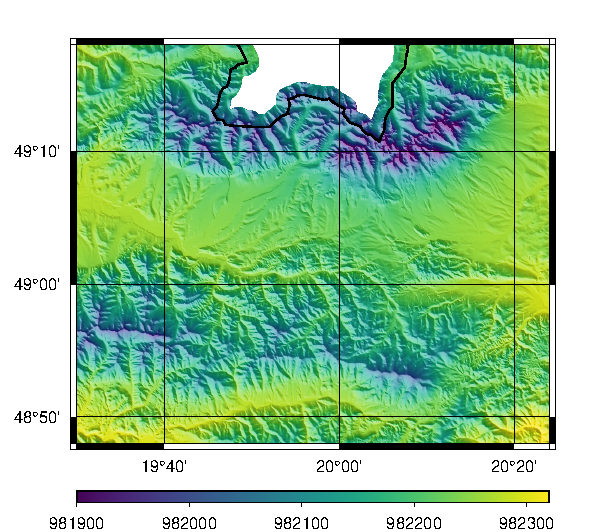
\includegraphics{./fig-gg-grav-sr-2arcsec.pdf}
\caption{Veľkosť vektora gravitačného zrýchlenia $| \vec g_\gidx |$ na zemskom 
povrchu v oblasti Vysokých a Nízkych Tatier (jednotky mGal).  Dáta prevzaté 
z modelu \texttt{grav-sr-2arcsec} \citep{GravSR2arcsec}}
\label{fig:gg_grav_sr_2arcsec}
\end{figure}

\begin{figure}
\centering
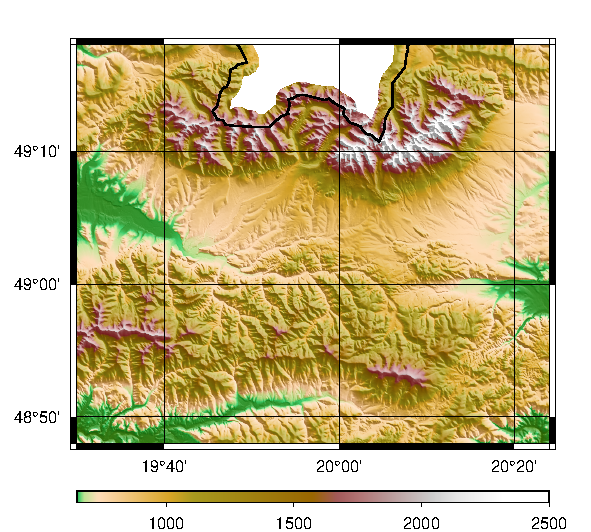
\includegraphics{./fig-h-grav-sr-2arcsec.pdf}
\caption{Topografia v oblasti Vysokých a Nízkych Tatier vyjadrená pomocou 
elipsoidickej výšky (jednotky~m).  Dáta prevzaté z modelu 
\texttt{grav-sr-2arcsec} \citep{GravSR2arcsec}}
\label{fig:h_grav_sr_2arcsec}
\end{figure}







\subsection{Gravitačný potenciál}
\label{sec:vg}

Gravitačné zrýchlenie $\vec g_\gidx$ je vektorová veličina, ktorá má v každom 
bode definovanú trojicu reálnych čísel,
%
\begin{equation}
\label{eq:gg_elements}
\vec g_{\gidx}(P) =
\begin{bmatrix}
g_{\gidx,x}(P) \\[2ex]
g_{\gidx,y}(P) \\[2ex]
g_{\gidx,z}(P)
\end{bmatrix}
{.}
\end{equation}
%
V niektorých situáciách je výhodnejšie pracovať so skalárnou veličinou, teda 
takou, ktorá má v bode~$P$ definované práve jedno reálne číslo.  Tento prístup 
je mladší ako Newtonov gravitačný zákon zhruba o jedno storočie 
\citep{MacMillan1930,Jekeli2015}.  Fenomén gravitácie chápe ako \emph{pole}, 
ktorého vlastnosti môžu byť popísané rôznymi vzájomne súvisiacimi veličinami, 
pričom však ide stále o to isté pole.  S konceptom potenciálu poľa prišiel 
podľa \cite{MacMillan1930} taliansky matematik a astronóm J. L. Lagrange 
(1736--1813).  Ak by sme teda našli skalárnu veličinu gravitačného poľa, 
informáciu poskytnutú troma číslami v podobe gravitačného vektora 
(vzťah~\ref{eq:gg_elements}) by sme dokázali zredukovať na jedno jediné číslo 
bez straty informácie o poli samotnom.  Skalárna veličina gravitačného poľa sa 
nazýva \emph{gravitačný potenciál} a označuje sa symbolom $V_\gidx$.

Gravitačný potenciál definujeme pomocou gravitačného zrýchlenia, ktoré, ako sme 
videli v predchádzajúcej časti, je definované pomocou gravitačnej sily 
vyplývajúcej z Newtonovho gravitačného zákona.  Pre lepšie pochopenie vzťahu 
medzi gravitačným zrýchlením a gravitačným potenciálom však najprv predstavíme 
diferenciálny operátor gradient a až následne pristúpime k samotnej definícii.

V trojrozmernom pravouhlom súradnicovom systéme $x$, $y$, $z$ je operátor 
gradient definovaný nasledovne,
%
\begin{equation}
\label{eq:gradient}
\nabla = \grad = \vec e_1 \frac{\partial}{\partial x} + \vec e_2 
\frac{\partial}{\partial y} + \vec e_3 \frac{\partial}{\partial z} =
\begin{bmatrix}
\dfrac{\partial}{\partial x} \\[2ex]
\dfrac{\partial}{\partial y} \\[2ex]
\dfrac{\partial}{\partial z}
\end{bmatrix}
{,}
\end{equation}
%
kde $\vec e_1$, $\vec e_2$ a $\vec e_3$ predstavujú jednotkové vektory 
rovnobežné so smerom súradnicových osí $x$, $y$ a $z$.  Aplikáciou operátora 
gradient na \emph{skalárnu} funkciu $f(x, y, z)$ získame \emph{vektorovú} 
funkciu,
%
\begin{equation}
\begin{split}
\vec f(x, y, z) &= \nabla f(x, y, z) = \grad \ f(x, y, z)\\
%
&= \vec e_1 \frac{\partial f(x, y, z)}{\partial x} + \vec e_2 \frac{\partial 
f(x, y, z)}{\partial y} + \vec e_3 \frac{\partial f(x, y, z)}{\partial z} =
\begin{bmatrix}
\dfrac{\partial f(x, y, z)}{\partial x} \\[2ex]
\dfrac{\partial f(x, y, z)}{\partial y} \\[2ex]
\dfrac{\partial f(x, y, z)}{\partial z}
\end{bmatrix}
{.}
\end{split}
\end{equation}
%
Vektorová funkcia $\vec f$ \emph{udáva smer a veľkosť najväčšieho nárastu} 
funkcie $f$ v bode so súradnicami $x$, $y$ a $z$.

Operátor gradient hrá v teórii fyzikálnych polí dôležitú úlohu, pretože 
umožňuje získať informácie o lokálnych charakteristikách poľa.  Medzi tieto 
informácie patrí smer a veľkosť najväčšieho nárastu funkcie, ale aj popis jej 
zmeny v smere súradnicových osí.  Vhodnou aplikáciou rotačných matíc je možné 
následne získať informáciu o zmene funkcie v ľubovoľnom smere, čo je v mnohých 
situáciách veľmi nápomocné.  Ak si predstavíme povrch Zeme ako dvojrozmernú 
funkciu zemepisnej šírky a dĺžky, potom aplikáciou operátora gradient na túto 
funkciu získame (nielen) v kopcovitom teréne informáciu o smere, ktorým sa 
z tohto bodu zrejme nechceme vydať na bicykli.  Ak však dáme pred vektorovú 
funkciu znamienko mínus, zvyšok práce môžeme nechať na gravitačné pole.  
Numerická ukážka aplikácie operátora gradient je spolu so zdrojovým kódom 
uvedená v Prílohe~\ref{app:numerical_application_of_gradient}.

Po tejto príprave môžeme definovať gravitačný potenciál nasledovne.  Gravitačný 
potenciál je skalárna funkcia, ktorá vyhovuje rovnici 
\citep{SansoGeoidDetermination}
%
\begin{equation}
\label{eq:gg_grad_vg}
\vec g_\gidx(P) = \nabla V_\gidx(P)
\end{equation}
%
a spĺňa podmienku
%
\begin{equation}
\label{eq:vg_at_infty}
\lim_{P \to \infty} V_\gidx(P) = 0{.}
\end{equation}
%
Vzťah~(\ref{eq:gg_grad_vg}) hovorí, že vektor gravitačného zrýchlenia udáva 
smer a veľkosť najväčšieho nárastu gravitačného potenciálu.  
Rovnica~(\ref{eq:vg_at_infty}) znamená, že gravitačný potenciál nadobúda 
v nekonečnej vzdialenosti od telesa nulovú hodnotu a zabezpečuje, že existuje 
práve jedna funkcia $V_\gidx$ vyhovujúca rovnici~(\ref{eq:gg_grad_vg}).  Keďže 
podmienka (\ref{eq:vg_at_infty}) bola definovaná (zvolená) dodatočne, 
\emph{gravitačný potenciál je relatívna veličina}.

Gravitačný potenciál hmotného bodu je daný nasledovne,
%
\begin{equation}
\label{eq:vg_point_mass}
V_\gidx(P) = \frac{G \, m}{l}{.}
\end{equation}
%
Overme, či tento vzťah vyhovuje rovniciam~(\ref{eq:gg_grad_vg}) 
a (\ref{eq:vg_at_infty}).  Aplikovaním operátora gradient~(\ref{eq:gradient}) 
na gravitačný potenciál~(\ref{eq:vg_point_mass}),
%
\begin{equation}
\label{eq:gg_from_vg_point_mass}
\nabla V_\gidx(P) = G \, m \, \nabla \left( \frac{1}{l} \right) =
%
G \, m
\begin{bmatrix}
\dfrac{\partial}{\partial x} \left( \dfrac{1}{l} \right)\\[2ex]
\dfrac{\partial}{\partial y} \left( \dfrac{1}{l} \right)\\[2ex]
\dfrac{\partial}{\partial z} \left( \dfrac{1}{l} \right)
\end{bmatrix}
%
=
%
-G \, m
%
\begin{bmatrix}
\dfrac{x - x_Q}{l^3}{,}\\[2ex]
\dfrac{y - y_Q}{l^3}{,}\\[2ex]
\dfrac{z - z_Q}{l^3}
\end{bmatrix}
{,}
\end{equation}
%
získame vektor gravitačného zrýchlenia $\vec g_\gidx(P)$ 
z rovnice~(\ref{eq:gg_point_mass}), čím bola dokázaná 
rovnosť~(\ref{eq:gg_grad_vg}).  Platnosť vzťahu~(\ref{eq:vg_at_infty}), teda
%
\begin{equation}
\lim_{l \to \infty} \frac{G \, m}{l} = 0{,}
\end{equation}
%
je zrejmá.

V sústave $N$ hmotných bodov je celkový gravitačný potenciál daný súčtom 
čiastkových príspevkov v dôsledku jednotlivých hmotných bodov,
%
\begin{equation}
\label{eq:vg_N_point_masses}
V_\gidx(P) = \sum_{i = 1}^{N} V_{\gidx,i}(P) = G \sum_{i = 1}^{N}\frac{
m_i}{l_i}{.}
\end{equation}
%
Obdobným spôsobom ako v rovnici~(\ref{eq:gg_from_vg_point_mass}) je možné 
presvedčiť sa, že aplikovaním operátora gradient na gravitačný 
potenciál~(\ref{eq:vg_N_point_masses}) získame vektor gravitačného 
zrýchlenia~(\ref{eq:gg_N_point_masses}).  Teda i v prípade gravitačného 
potenciálu generovaného sústavou $N$ hmotných bodov sú 
rovnice~(\ref{eq:gg_grad_vg}) a (\ref{eq:vg_at_infty}) splnené.

Od gravitačného potenciálu, ktorý je generovaný $N$ hmotnými bodmi prejdeme ku 
gravitačnému potenciálu všeobecného telesa podobnou úvahou ako 
v Kapitole~\ref{sec:gg}.  Teleso rozdelíme na diferenciálne hmotné elementy 
$\diff m$ a gravitačný potenciál získame integráciou,
%
\begin{equation}
\label{eq:vg_body}
V_\gidx(P) = G \iiint_{\tau} \frac{\rho}{l} \diff\tau{.}
\end{equation}
%
Dôkaz, že i rovnica~(\ref{eq:vg_body}) vyhovuje prijatej definícii gravitačného 
potenciálu (\ref{eq:gg_grad_vg} a \ref{eq:vg_at_infty}) vynecháme, no je 
dostupný napríklad v \cite{MacMillan1930}.

K interpretácii gravitačného potenciálu je možné pristúpiť aj z fyzikálneho 
hľadiska.  Bez podrobného odvodenia sa obmedzíme na tvrdenie, že hodnota 
gravitačného potenciálu v bode $P$ predstavuje prácu, ktorú musí vykonať 
gravitačné pole pri premiestnení hmotného bodu s hmotnosťou $1\ \mathrm{kg}$ 
z miesta s nulovým potenciálom (v geodézii nekonečno, pozri 
vzťah~\ref{eq:vg_at_infty}) do bodu $P$ 
\citep{MacMillan1930,Kellogg1967,TorgeGeodesy}.  \emph{Práca} je dráhový účinok 
sily, v tomto prípade gravitačnej.  Gravitačná sila má tú vlastnosť, že práca 
spôsobená jej silovým účinkom \emph{nezávisí} od dráhy, dôležitý je iba 
začiatočný a koncový bod dráhy.  Ak sú začiatočný a koncový bod totožné, práca 
je nulová.  Bez tejto vlastnosti by nebolo možné nájsť skalárnu funkciu 
$V_\gidx$, ktorá by vyhovovala rovnici~(\ref{eq:gg_grad_vg}).

Na rozdiel od vektora gravitačného zrýchlenia, gravitačný potenciál nedokážeme 
priamo merať.  Vo fyzikálnej geodézii vystupuje často ako neznáma funkcia, 
ktorú sa snažíme určiť, napríklad z vektora gravitačného zrýchlenia.  V sústave 
SI má gravitačný potenciál fyzikálnu jednotku $\mathrm{m}^2\ \mathrm{s}^{-2}$.  
Ukážka priebehu gravitačného potenciálu v oblasti Vysokých a Nízkych Tatier je 
uvedená na Obrázku~\ref{fig:vg_grav_sr_2arcsec}.

\begin{figure}
\centering
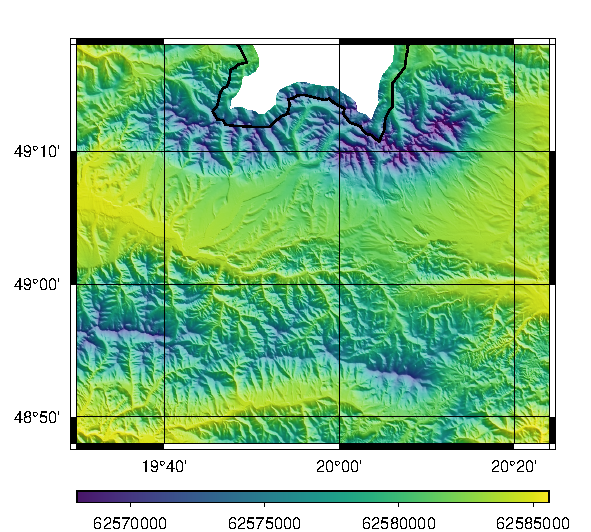
\includegraphics{./fig-vg-grav-sr-2arcsec.pdf}
\caption{Gravitačný potenciál $V_\gidx$ na zemskom povrchu v oblasti Vysokých 
a Nízkych Tatier (jednotky $\mathrm{m}^2 \ \mathrm{s}^{-2}$).  Dáta prevzaté 
z modelu \texttt{grav-sr-2arcsec} \citep{GravSR2arcsec}}
\label{fig:vg_grav_sr_2arcsec}
\end{figure}






\section{Teória potenciálu}
\label{sec:potential_theory}

Rovnica~(\ref{eq:vg_body}) sa v literatúre zvykne nazývať \emph{Newtonov 
integrál}.  Hovorí, že ak poznáme tvar a priestorové rozloženie hustoty telesa, 
gravitačný potenciál generovaný týmto telesom môže byť vypočítaný.  Newtonov 
integrál má vo fyzikálnej geodézii kľúčový význam, nakoľko v gravitačnom 
potenciáli je obsiahnutá informácia o celom gravitačnom poli (pozri 
Kapitolu~\ref{sec:newton_law}).

Newtonov integrál položil základy novej oblasti matematiky a matematickej 
fyziky s názvom \emph{teória potenciálu}.  Podľa \cite{MacMillan1930} siahajú 
jej začiatky k francúzskemu matematikovi, fyzikovi, astronómovi a politikovi 
P. S. Laplaceovi (1749--1827).  Ten si uvedomil, že gravitačný potenciál 
každého všeobecného telesa (v zmysle definície z Kapitoly~\ref{sec:gg}) spĺňa 
určité podmienky, čím vzniká zaujímavá množina funkcií hodná podrobnejšieho 
štúdia.  Významnosť teórie potenciálu iba potvrdzuje skutočnosť známa približne 
od čias C. F. Gaussa, a síce že túto teóriu je možné aplikovať nielen na 
gravitačné pole, ale  napríklad aj na magnetické, či elektrostatické pole 
(spomeňme si na Coulombov zákon a porovnajme ho s Newtonovým gravitačným 
zákonom~\ref{eq:newton_law}).  Teória potenciálu teda študuje 
vzťah~(\ref{eq:vg_body}) vo všeobecnom zmysle, pričom sa zaoberá rozličnými 
zdrojmi poľa (hmotný bod, hmotná priamka, nekonečne tenká vrstva, všeobecné 
teleso a pod.) s rôznym priestorovým rozložením hustôt (konštantná, premenlivá, 
kladná, dokonca i záporná a pod.) a neobmedzuje sa iba na gravitačné pole.  
Táto úloha je nesmierne náročná.  Čo sa napríklad stane v prípade, ak 
v rovnici~(\ref{eq:vg_body}) sa nachádza výpočtový bod $P$ vo vnútri telesa?  
Za takýchto okolností musí nevyhnutne dôjsť k situácii, v ktorej súradnice bodu 
$P$, kde je hľadaný gravitačný potenciál, sú identické so súradnicami jedného 
diferenciálneho hmotného elementu $\diff m$.  Vzájomná vzdialenosť medzi bodom 
$P$ a elementom $\diff m$ vystupujúca v menovateli bude teda $l = 0$.  
Konverguje alebo diverguje v takejto situácii integrál~(\ref{eq:vg_body})?  
Jednou z mnohých ďalších výziev sú gravitačné polia generované objektmi 
komplikovaného tvaru, napríklad s náhlymi ostrými zmenami tvaru ako je tomu 
v prípade zemského povrchu.  Je preto prirodzené, že tieto matematické výzvy 
pritiahli záujem brilantných matematikov akými boli, okrem iných, 
J. L. Lagrange, P. S. Laplace, britský samouk G. Green (1793--1841), či 
C. F. Gauss.

V nasledujúcich troch kapitolách (\ref{sec:laplace_equation}~-- 
\ref{sec:poisson_equation}) sa budeme zaoberať niektorými základnými 
vlastnosťami gravitačného potenciálu, ktoré vyplývajú z teórie potenciálu.  
Vlastnosti budú popísané pre gravitačný potenciál mimo telesa a vo vnútri 
telesa.





\subsection{Laplaceova rovnica}
\label{sec:laplace_equation}

P. S. Laplace zistil, že gravitačný potenciál každého všeobecného telesa spĺňa 
v bode $P(x, y, z)$ \emph{mimo} tohto telesa rovnicu
%
\begin{equation}
\label{eq:vg_laplace_cart}
\nabla^2 V_\gidx = \Delta V_\gidx = \frac{\partial^2 V_\gidx}{\partial x^2}
+ \frac{\partial^2 V_\gidx}{\partial y^2} + \frac{\partial^2 V_\gidx}{\partial 
z^2} = 0{.}
\end{equation}
%
Operátor $\nabla^2 = \Delta$ sa nazýva \emph{Laplaceov operátor} 
a rovnica~(\ref{eq:vg_laplace_cart}) na nazýva \emph{Laplaceova rovnica} pre 
gravitačný potenciál.  Laplaceov operátor je \emph{lineárny}, teda pre funkcie 
$f$ a $g$ vyhovujúce rovnici~(\ref{eq:vg_laplace_cart}) a konštantu $c$ platí
%
\begin{equation}
\label{eq:laplace_additivity}
\nabla^2 \left(f + g \right) = \nabla^2 f + \nabla^2 g
\end{equation}
%
a
%
\begin{equation}
\label{eq:laplace_homogenity}
\nabla^2 (c \, f) = c \, \nabla^2 f{.}
\end{equation}

Skúsme overiť, či gravitačný potenciál hmotného bodu~(\ref{eq:vg_point_mass}) 
vyhovuje Laplaceovej rovnici.  Budeme uvažovať, že $l > 0$, nakoľko gravitačný 
potenciál hmotného bodu nie je definovaný pre $l = 0$.  
S uvážením~(\ref{eq:laplace_homogenity}), postačuje dokázať, že
%
\begin{equation}
\label{eq:nabla_l}
\nabla^2 \left( \frac{1}{l} \right) = 0{,}
\end{equation}
%
pretože $G \, m$ je konštanta, teda $G \, m = c$.  Vypočítajme teda druhé 
parciálne derivácie funkcie $1 \slash l$,
%
\begin{equation}
\label{eq:l_2nd_derivatives}
\begin{split}
\frac{\partial^2}{\partial x^2} \left( \frac{1}{l} \right) &= 
-\frac{\partial}{\partial x} \left( \frac{x - x_Q}{l^3} \right) = \left(3 
\frac{(x - x_Q)^2}{l^5} - \frac{1}{l^3} \right){,}\\
%
\frac{\partial^2}{\partial y^2} \left( \frac{1}{l} \right) &= 
-\frac{\partial}{\partial y} \left( \frac{y - y_Q}{l^3} \right) = \left(3 
\frac{(y - y_Q)^2}{l^5} - \frac{1}{l^3} \right){,}\\
%
\frac{\partial^2}{\partial z^2} \left( \frac{1}{l} \right) &= 
-\frac{\partial}{\partial z} \left( \frac{z - z_Q}{l^3} \right) = \left(3 
\frac{(z - z_Q)^2}{l^5} - \frac{1}{l^3} \right){.}
\end{split}
\end{equation}
%
Súčet členov na pravej strane predošlých troch rovníc je nulový, čím bolo 
dokázané, že gravitačný potenciál hmotného bodu vyhovuje Laplaceovej 
diferenciálnej rovnici~(\ref{eq:vg_laplace_cart}) pre $l > 0$.

Využitím vzťahov~(\ref{eq:l_2nd_derivatives}) a vlastností Laplaceovho 
operátora~(\ref{eq:laplace_additivity}) a (\ref{eq:laplace_homogenity}) je 
možné presvedčiť sa, že Laplaceovej rovnici vyhovuje i gravitačný potenciál 
generovaný sústavou $N$ hmotných bodov,
%
\begin{equation}
\nabla^2 \left( \sum_{i = 1}^N V_{\gidx,i} \right) = \sum_{i = 1}^N \nabla^2 
V_{\gidx,i} = 0{,}
\end{equation}
%
ako aj gravitačný potenciál všeobecného telesa v bode \emph{mimo telesa},
%
\begin{equation}
\nabla^2 V_\gidx = G\, \iiint_\tau \rho \, \left[ \frac{\partial^2}{\partial 
x^2}\left(\frac{1}{l}\right) + \frac{\partial^2}{\partial 
y^2}\left(\frac{1}{l}\right) + \frac{\partial^2}{\partial 
z^2}\left(\frac{1}{l}\right) \right] \diff\tau = 0{.}
\end{equation}

Podľa \cite{MacMillan1930} Laplace predstavil 
rovnicu~(\ref{eq:vg_laplace_cart}) po prvýkrát nie v pravouhlých súradniciach 
$x$, $y$ a $z$, ale vo sférických súradniciach,
%
\begin{equation}
\label{eq:vg_laplace_sph}
\nabla^2 V_\gidx = \frac{1}{r^2} \frac{\partial}{\partial r} \left( r^2 
\frac{\partial V_\gidx}{\partial r} \right) + \frac{1}{r^2 \, \cos\varphi} 
\frac{\partial}{\partial \varphi} \left( \cos\varphi \frac{\partial 
V_\gidx}{\partial \varphi} \right) + \frac{1}{r^2 \, 
\cos^2\varphi}\frac{\partial^2 V_\gidx}{\partial \lambda^2} = 0{,}
\end{equation}
%
kde $r$ je sprievodič, $\varphi$ je sférická šírka a $\lambda$ je sférická 
dĺžka bodu $P$ (Obrázok~\ref{fig:cart_sph}).  Existuje tiež všeobecný zápis 
Laplaceovej rovnice v ľubovoľných pravouhlých súradniciach \citep[pozri 
napríklad][]{MoritzPhysicalGeodesy}.

\begin{figure}
\centering
\input{./fig-cart-sph.pdf_tex}
\caption{Pravouhlé a sférické súradnice bodu $P$}
\label{fig:cart_sph}
\end{figure}






\subsection{Harmonická funkcia}

Laplaceovej rovnici vyhovuje nielen gravitačný potenciál mimo telesa, ale 
nekonečné množstvo funkcií.  Zaveďme preto pojem \emph{harmonická funkcia}.  
Harmonická funkcia je taká funkcia, ktorá má spojité prvé a druhé parciálne 
derivácie na otvorenej množine $\Omega$ a vyhovuje Laplaceovej rovnici
%
\begin{equation}
\nabla^2 f = 0
\end{equation}
%
v každom bode oblasti $\Omega$.

Každá harmonická funkcia je \emph{analytická} v oblasti, v ktorej vyhovuje 
Laplaceovej rovnici \citep{MoritzPhysicalGeodesy}.  To znamená, že každá 
harmonická funkcia je spojitá, má spojité všetky derivácie a v každom bode 
oblasti $\Omega$ ju možno rozvinúť do mocninového radu (napríklad Taylorovho), 
ktorý konverguje.  Táto vlastnosť je dôležitá, preto sa pri nej na chvíľku 
pristavme.

Uvažujme všeobecné teleso generujúce gravitačné pole.  Nech sú dané dva body, 
$P_1(r, \varphi, \lambda)$ a $P_2(r + \Delta r, \varphi, \lambda)$, $\Delta 
r > 0$, nachádzajúce sa mimo tohto telesa a na tej istej spojnici so začiatkom 
súradnicového systému, ktorý sa nachádza v ťažisku telesa 
(Obrázok~\ref{fig:analytical_continuation}).  Keďže gravitačný potenciál mimo 
telesa je harmonická, a teda analytická, funkcia, môžeme ho v bode $P_1$ 
rozvinúť do Taylorovho radu, ktorý konverguje,
%
\begin{equation}
\label{eq:vg_analytical_continuation}
V_\gidx(P_2) = \sum_{i = 0}^\infty \frac{1}{i!} \, \frac{\partial^i 
V_\gidx(P_1)}{\partial r^i} \, \Delta r^i{.}
\end{equation}

\begin{figure}
\centering
\input{./fig-analytical-continuation.pdf_tex}
\caption{Analytické pokračovanie gravitačného poľa z bodu $P_1$ do bodu $P_2$}
\label{fig:analytical_continuation}
\end{figure}

Rovnica~(\ref{eq:vg_analytical_continuation}) hovorí, že z lokálnych vlastností 
gravitačného potenciálu, ktoré sú obsiahnuté v deriváciách $\partial^i V_\gidx 
\slash \partial r^i$, dokážeme určiť hodnotu gravitačného potenciálu 
v ľubovoľnom bode v radiálnom smere pre $\Delta r > 0$.  Tento proces sa nazýva 
\emph{analytické pokračovanie} gravitačného potenciálu.  Čím väčšia vzdialenosť 
$\Delta r$ na ktorú predikujeme gravitačný potenciál, tým pomalšie 
rad~(\ref{eq:vg_analytical_continuation}) konverguje a naopak.  Analyticky 
pokračovať je možné aj v iných smeroch ako v radiálnom.  V takom prípade je 
potrebné derivovať gravitačný potenciál v príslušnom smere.  Rovnako tak je 
možné analyticky pokračovať aj iné veličiny gravitačného poľa, napríklad vektor 
gravitačného zrýchlenia,
%
\begin{equation}
\vec g_\gidx(P_2) = \sum_{i = 0}^{\infty} \frac{1}{i!} \, \frac{\partial^i \vec 
g_\gidx(P_1)}{\partial r^i} \, \Delta r^i{.}
\end{equation}

Na záver dodajme, že situácia je výrazne komplikovanejšia, ak analyticky 
pokračujeme z bodu $P_2$ do bodu $P_1$.  Táto úloha je zvyčajne zle podmienená 
\citep{SansoGeodeticBoundaryValueProblem}.  V praktických numerických 
aplikáciách to znamená, že i malá chyba vo vstupných dátach spôsobuje veľké 
chyby vo výsledkoch.  Takáto úloha sa nazýva \emph{numericky nestabilná}.  






\subsection{Poissonova rovnica}
\label{sec:poisson_equation}

Z Kapitoly~\ref{sec:laplace_equation} vieme, že Laplaceova rovnica pre 
gravitačný potenciál platí v každom bode mimo telesa.  \emph{Vo vnútri} telesa 
platí \emph{Poissonova rovnica},
%
\begin{equation}
\label{eq:vg_poisson_equation}
\nabla^2 V_\gidx(P) = -4 \pi \, G \, \rho(P){,}
\end{equation}
%
kde $\rho(P)$ je hustota v bode $P$.  Odvodenie Poissonovej rovnice je možné 
nájsť napríklad v \cite{MacMillan1930}, \cite{Kellogg1967} či 
\cite{SansoGeoidDetermination}.

Poissonovu rovnicu je možné vnímať ako zovšeobecnenie Laplaceovej rovnice.  Ak 
sa bod $P$ vo vzťahu~(\ref{eq:vg_poisson_equation}) nachádza mimo telesa 
generujúceho potenciál, potom $\rho(P) = 0$, čím dostávame Laplaceovu 
rovnicu~(\ref{eq:vg_laplace_cart}).

Posledná oblasť, v ktorej sa môže nachádzať bod $P$, no nie je pokrytá ani 
Laplaceovou, ani Poissonovou rovnicou, je \emph{povrch} telesa.  Vo 
všeobecnosti, druhé derivácie gravitačného potenciálu vystupujúce v operátore 
$\nabla^2$ (pozri rovnice~\ref{eq:vg_laplace_cart} a \ref{eq:vg_laplace_sph}) 
nie sú v takom prípade definované \citep{Kellogg1967}.  Dôvodom je nespojitosť 
hustoty $\rho$, ktorá sa na povrchu mení z $\rho \neq 0$ na 0, resp. naopak, 
v závislosti od smeru prechodu.






\section{Odstredivé pole a tiažové pole}
\label{sec:centrifugal_gravity_field}

Newtonov gravitačný zákon~(\ref{eq:newton_law}) platí v súradnicovom systéme, 
ktorý je v pokoji alebo je v stave rovnomerného priamočiareho pohybu.  Takýto 
súradnicový systém sa nazýva \emph{inerciálny súradnicový systém}.

Uvažujme súradnicový systém so začiatkom v ťažisku Zeme a s osou $z$, ktorá je 
totožná s rotačnou osou Zeme.  Nech tento súradnicový systém rotuje spolu so 
Zemou uhlovou rýchlosťou $\omega$.  Takýto súradnicový systém nie je 
inerciálny, pretože vzhľadom na inerciálny súradnicový systém v ňom dochádza 
prinajmenšom k dvom nelineárnym pohybom.  Prvý vzniká v dôsledku rotácie Zeme 
okolo vlastnej osi, druhý je spôsobený obehom Zeme okolo Slnka.  Ak teda chceme 
študovať sily pôsobiace na Zemi v takomto neinerciálnom súradnicovom systéme, 
potrebné je uvážiť nielen gravitačnú silu, ale i ďalšie sily v zmysle 
Newtonovho pohybového zákona.  Na objekt, ktorý sa nachádza na rotujúcej Zemi 
a je vzhľadom k nej v pokoji pôsobí okrem gravitačnej sily aj \emph{odstredivá 
sila}.  Ak je objekt v pohybe, pôsobí naň i tretia sila, ktorá sa nazýva 
\emph{Coriolisova sila}.  Azda väčšina meracích geodetických zariadení je počas 
merania v pokoji vzhľadom k Zemi, preto Coriolisovu silu nebudeme ďalej 
uvažovať.  Spomeňme tiež, že ak sa uhlová rýchlosť rotácie $\omega$ mení 
v čase, potrebné je uvážiť i \emph{Eulerovu silu}.  Tieto tri sily, odstredivá, 
Coriolisova a Eulerova, sa zaraďujú medzi \emph{zotrvačné sily}, niekedy tiež 
nazývané fiktívne sily, a nevznikajú vzájomným silovým pôsobením medzi objektmi 
ako je tomu v prípade gravitačnej sily.






\subsection{Odstredivé a tiažové zrýchlenie}

Najvýznamnejšia zotrvačná sila vo fyzikálnej geodézii je \emph{odstredivá sila} 
$\vec F_\cidx$.  Uvažujme súradnicový systém v zmysle predošlého odseku 
a hmotný bod $P(x, y, z)$ s hmotnosťou $1\ \mathrm{kg}$.  V neinerciálnom 
súradnicovom systéme pôsobí na hmotný bod $P$ \emph{odstredivé zrýchlenie}.  
Odstredivé zrýchlenie v bode $P$ budeme označovať symbolom $\vec g_\cidx(P)$ 
a je dané vzťahom
%
\begin{equation}
\label{eq:gc}
\vec g_\cidx(P) = \omega^2 \, \vec p =
%
\begin{bmatrix}
\omega^2 \, x\\
\omega^2 \, y\\
0
\end{bmatrix}
{.}
\end{equation}
%
Za predpokladu konštantnej uhlovej rýchlosti rotácie $\omega$ teda závisí 
veľkosť odstredivého zrýchlenia iba od vzdialenosti $p = | \vec p |$ bodu $P$ 
od rotačnej osi (Obrázok~\ref{fig:gravity_vector}),
%
\begin{equation}
| \vec g_\cidx | = \omega^2 \, p = \omega^2 \, \sqrt{x^2 + y^2}{.}
\end{equation}
%
Čím je vzdialenosť $p$ väčšia, tým je väčšie i odstredivé zrýchlenie a naopak.  
Zo vzťahu~(\ref{eq:gc}) je zrejmé, že odstredivé zrýchlenie je kolmé na os 
rotácie a má smer vzdiaľujúci sa od rotačnej osi 
(Obrázok~\ref{fig:gravity_vector}).  Uhlová rýchlosť rotácie Zeme je približne 
rovná \citep{GRS80}
%
\begin{equation}
\omega = 7\, 292\, 115 \times 10^{-11} \ \mathrm{rad} \ \mathrm{s}^{-1}{.}
\end{equation}

\begin{figure}
\centering
\input{./fig-gravity-vector.pdf_tex}
\caption{Vektory gravitačného $\vec g_\gidx$, odstredivého $\vec g_\cidx$ 
a tiažového zrýchlenia $\vec g$ v bode $P$ na povrchu idealizovanej rotujúcej 
Zeme sférického tvaru a konštantnej hustoty}
\label{fig:gravity_vector}
\end{figure}

Výsledné zrýchlenie pôsobiace na hmotný bod s hmotnosťou $1 \ \mathrm{kg}$ je 
v neinerciálnom systéme dané súčtom gravitačnej a odstredivej 
sily.\footnote{Ostatné sily sme pre túto chvíľu s rozumnou mierou aproximácie 
zanedbali.}  Toto zrýchlenie sa nazýva \emph{tiažové zrýchlenie}, označuje sa 
symbolom $\vec g(P)$ a je možné vypočítať ho vektorovým súčtom 
gravitačného~(\ref{eq:gg_body}) a odstredivého~(\ref{eq:gc}) zrýchlenia 
(Obrázok~\ref{fig:gravity_vector}),
%
\begin{equation}
\label{eq:g}
\vec g(P) = \vec g_\gidx(P) + \vec g_\cidx(P){.}
\end{equation}

Vektor tiažového zrýchlenia je možné odmerať, a tak predstavuje ústrednú 
veličinu v procese určovania tvaru Zeme.  Prístroj, ktorým sa meria veľkosť 
vektora tiažového zrýchlenia $| \vec g |$ sa nazýva \emph{gravimeter}.  
V súčasnosti bežne dosiahnuteľná presnosť určenia $| \vec g |$ dosahuje hodnotu 
niekoľkých mikroGalov.  Smer vektora tiažového zrýchlenia je možné odmerať 
astronomickým určením zemepisnej šírky a zemepisnej dĺžky daného bodu $P$.  
Presnosť astronomických súradníc sa v súčasnosti pohybuje v desatinách uhlovej 
sekundy.






\subsection{Odstredivý a tiažový potenciál}

Podobne ako v prípade gravitačného poľa, i odstredivé a tiažové zrýchlenie je 
možné definovať pomocou skalárnych veličín.  Tieto skalárne veličiny sa 
nazývajú \emph{odstredivý potenciál},
%
\begin{equation}
\label{eq:vc}
V_c(P) = \frac{1}{2} \, \omega^2 \, (x^2 + y^2){,}
\end{equation}
%
a \emph{tiažový potenciál},
%
\begin{equation}
\label{eq:w}
W(P) = V_\gidx(P) + V_\cidx(P){.}
\end{equation}
%
Príslušné zrýchlenia~(\ref{eq:gc}) a (\ref{eq:g}) získame aplikovaním operátora 
gradient na tieto rovnice,
%
\begin{equation}
\label{eq:gc_vc}
\vec g_\cidx(P) = \nabla V_c(P)
\end{equation}
%
a
%
\begin{equation}
\label{eq:g_gradW}
\vec g(P) = \nabla W(P) = \nabla V_\gidx(P) + \nabla V_\cidx(P) = \vec 
g_\gidx(P) + \vec g_\cidx(P){.}
\end{equation}
%
V zmysle vlastností operátora gradient (Kapitola~\ref{sec:vg}), vektory $\vec 
g_\cidx(P)$ a $\vec g(P)$ udávajú veľkosť a smer najväčšieho nárastu 
odstredivého a tiažového potenciálu $V_\cidx(P)$ a $W(P)$ v bode $P$.  Platnosť 
rovnice~(\ref{eq:gc_vc}) možno overiť pomocou~(\ref{eq:gradient}) 
a (\ref{eq:vc}), čím získame (\ref{eq:gc}).  V rovnici~(\ref{eq:g_gradW}) bola 
využitá skutočnosť, že \emph{operátor gradient je lineárny}, teda tie isté 
vlastnosti ako pre Laplaceov operátor, (\ref{eq:laplace_additivity}) 
a (\ref{eq:laplace_homogenity}), platia aj pre operátor gradient.

Odstredivý ani tiažový potenciál nedokážeme priamo odmerať, podobne ako 
nedokážeme priamo odmerať gravitačný potenciál.  V sústave SI majú odstredivý 
a tiažový potenciál jednotky $\mathrm{m}^2 \ \mathrm{s}^{-2}$.

\subsubsection{Ekvipotenciálna plocha}

Plocha, na ktorej je hodnota tiažového potenciálu $W$ konštantná sa nazýva 
\emph{ekvipotenciálna plocha} (Obrázok~\ref{fig:equipotential_surfaces}).  
V úvodnej kapitole jeden z prístupov definuje tvar Zeme ako geoid, teda tú 
ekvipotenciálnu plochu, ktorá koinciduje s hladinou morí a oceánov.  Pre 
fyzikálnu geodéziu majú preto ekvipotenciálne plochy veľký význam.  Zamerajme 
sa na niektoré ich vlastnosti.

\begin{figure}
\centering
\input{./fig-equipotential-surfaces.pdf_tex}
\caption{Ekvipotenciálne plochy s konštantným krokom tiažového potenciálu 
$\Delta W$}
\label{fig:equipotential_surfaces}
\end{figure}

\begin{itemize}
\item Ekvipotenciálne plochy sú spojité.  Táto vlastnosť vyplýva zo 
skutočnosti, že gravitačný potenciál~(\ref{eq:vg_body}), a teda i tiažový 
potenciál~(\ref{eq:w}), je spojitou funkciou v celom priestore 
\citep{Janak2006}.

\item Ekvipotenciálne plochy sú uzavreté \citep{VanicekGeodesy}.

\item Ekvipotenciálne plochy mimo telesa sú analytickými plochami.  
Ekvipotenciálne plochy, ktoré sa celé nachádzajú vo vnútri telesa alebo ho 
pretínajú nie sú analytické, pretože ich krivosť sa môže meniť nespojito 
v závislosti od hustoty \citep{MoritzPhysicalGeodesy}.

\item Všetky ekvipotenciálne plochy sú hladké a neobsahujú hrany 
\citep{MoritzPhysicalGeodesy}.

\item Ekvipotenciálne plochy sa nepretínajú.  Tiažový potenciál $W$ má v každom 
bode definované práve jedno číslo (skalárna veličina), preto sa ekvipotenciálne 
plochy nemôžu pretnúť \citep{MacMillan1930}.

\item Vektor tiažového zrýchlenia v ľubovoľnom bode je kolmý na ekvipotenciálnu 
plochu prechádzajúcu týmto bodom \citep{MoritzPhysicalGeodesy}.  Toto tvrdenie 
vyplýva priamo z rovnice~(\ref{eq:g_gradW}).
\end{itemize}

Matematický popis tvaru ekvipotenciálnych plôch realných telies je náročný.  
Z Newtonovho integrálu~(\ref{eq:vg_body}) vieme (pozri tiež 
Kapitolu~\ref{sec:potential_theory}), že sú to tvar a hustota telesa, ktoré 
definujú jeho gravitačné pole.  Zložité nepravidelné tvary či rozloženia 
hustoty majú za následok zvlnenia ekvipotenciálnych plôch od ideálneho 
sférického tvaru.\footnote{Na tvar ekvipotenciálnych plôch vplýva aj odstredivý 
potenciál $V_\cidx$ (vzťah~\ref{eq:w}).  Ten sa mení so zmenou uhlovej 
rýchlosti rotácie telesa a so zmenou polohy bodu voči osi rotácie.  V prípade 
Zeme má variácia týchto parametrov výrazne menší vplyv na tvar 
ekvipotenciálnych plôch ako tvar a hustota Zeme, preto tieto effekty pre túto 
chvíľu zanedbajme.}  Na regionálnej úrovni je nepravidelný tvar 
ekvipotenciálnych plôch do veľkej miery spôsobený lokálnymi hmotami, napríklad 
pohoriami.  Z globálneho pohľadu je tvar ekvipotenciálnych plôch daný skôr 
celkovou geometriou telesa ako takého (napríklad sploštenie Zeme) či 
rozsiahlymi hustotnými kontrastami.  Práve tieto skutočnosti výrazne komplikujú 
presný výpočet geoidu, jednej ekvipotenciálnej plochy z nekonečného množstva 
ekvipotenciálnych plôch.  Podrobnejší popis niektorých dôležitých vlastností 
ekvipotenciálnych plôch, napríklad ich krivostí, je možne nájsť napríklad 
v \cite{Janak2006} či v \cite{MoritzPhysicalGeodesy}.

Obrázok~\ref{fig:equipotential_surfaces} schematicky znázorňuje ekvipotenciálne 
plochy tiažového poľa Zeme s konštantným krokom tiažového potenciálu $\Delta 
W$.  Možno si všimnúť, že priestorový rozostup ekvipotenciálnych plôch je väčší 
v rovníkových oblastiach ako v polárnych oblastiach.  Malý rozostup 
ekvipotenciálnych plôch znamená veľkú zmenu tiažového poľa a naopak.  Veľkosť 
vektora tiažového zrýchlenia $| \vec g |$ je teda väčšia v oblasti pólov ako 
v oblasti rovníka.

Horizontovaním geodetického prístroja zabezpečujeme, že jeho horizontálna 
rovina je dotyková k ekvipotenciálnej ploche, ktorá prechádza stredom libely.  
Z dôvodu sférického tvaru Zeme a zvlnenia ekvipotenciálnych plôch nemožno vo 
všeobecnosti predpokladať rovnobežnosť horizontálnych rovín na dvoch rôznych 
stanoviskách.  V prípade teodolitu sú v tejto rovine merané vodorovné smery.  
Preto ak je vyžadovaná presnosť vysoká alebo záujmová lokalita je rozsiahla 
a má zložitú topografiu, potrebné je korigovať merania o vplyv nerovnobežnosti 
horizontálnych rovín medzi stanoviskami.

\subsubsection{Tiažnica}

Siločiara tiažového poľa sa nazýva \emph{tiažnica}.  Tiažnica je priestorová 
krivka kolmá na všetky ekvipotenciálne plochy 
(Obrázok~\ref{fig:equipotential_surfaces}).  Dotyčnica k tiažnici sa nazýva 
\emph{zvislica}.  Smer zvislice je daný smerom vektora tiažového zrýchlenia.  
V geodézii sa tiažnice využívajú napríklad na definovanie fyzikálnych 
(nadmorských) výšok.  Jedna taká výška má názov \emph{ortometrická výška} a je 
meraná pozdĺž tiažnice od geoidu po bod $P$ (pozri 
Obrázok~\ref{fig:equipotential_surfaces}).

Z pohľadu geodetických meraní je nutné, aby zvislá os prístroja (napríklad 
teodolitu) bola totožná s lokálnou zvislicou.  Táto podmienka je splnená po 
zhorizontovaní prístroja za predpokladu, že horizontálna os prístroja je kolmá 
na jeho vertikálnu os.  K lokálnej zvislici sa vzťahujú napríklad merané 
vertikálne smery.  Sférický tvar Zeme a zvlnenie ekvipotenciálnych plôch 
spôsobujú, že vertikálne osi zhorizontovaných prístrojov nie sú vo všeobecnosti 
rovnobežné medzi stanoviskami.  Podobne ako pri vodorovných smeroch, presné 
merania si môžu vyžadovať zavedenie korekcii.






\section{Gravitačné a tiažové pole homogénnej gule}





% -----------------------------------------------------------------------------

\chapter{Sférické harmonické funkcie}
\label{sec:spherical_harmonics}

Newtonov integrál~(\ref{eq:vg_body}) nie je vhodný na priamy praktický výpočet 
gravitačného poľa Zeme.  Predpokladá totiž, že poznáme dve matematické funkcie: 
jednu, ktorá definuje tvar telesa a druhú, ktorá opisuje jeho hustotu.  
Problematická je obzvlášť hustota.  Hoci existujú hustotné modely Zeme 
\citep[napríklad][]{Dziewonski1981}, ich použitie vo vzťahu~(\ref{eq:vg_body}) 
ešte stále neposkytuje vyžadovanú geodetickú presnosť.  V tejto situácii nie sú 
postačujúce ani regionálne hustotné modely.  Hoci tie poskytujú vyššiu presnosť 
a priestorové rozlíšenie, v geodézii sa používajú prevažne ako cenná doplnková 
informácia o zdroji gravitačného poľa, nie však ako hlavné dáta na výpočet 
tiažového poľa Zeme.  V tejto kapitole sa zameriame na praktický spôsob 
modelovania gravitačného poľa Zeme \emph{bez potreby priamej znalosti hustoty}.  
Pred samotným predstavením metódy však skúsme ilustrovať jej základnú myšlienku 
a širší kontext.






\section{Jednotkové vektory v trojrozmernom pravouhlom súradnicovom systéme}

Nech je daný trojrozmerný pravouhlý súradnicový systém so začiatkom v bode $O$ 
a so súradnicovými osami $x$, $y$ a $z$.  Označme symbolmi $\vec e_1$, $\vec 
e_2$ a $\vec e_3$ jednotkové vektory v smere týchto súradnicových osí,
%
\begin{equation}
\vec e_1 =
\begin{bmatrix}
1\\
0\\
0\\
\end{bmatrix}
{,} \quad
%
\vec e_2 =
\begin{bmatrix}
0\\
1\\
0
\end{bmatrix}
%
{,}\quad
%
\vec e_3 =
\begin{bmatrix}
0\\
0\\
1
\end{bmatrix}
{.}
\end{equation}
%
Nech symbol $\vec r$ predstavuje ľubovoľný vektor v tomto priestore,

\begin{figure}
\centering
\input{./fig-unit-vectors.pdf_tex}
\caption{Jednotkové vektory $\vec e_1$, $\vec e_2$, $\vec e_3$ trojrozmerného 
pravouhlého súradnicového systému a polohový vektor $\vec r$ bodu $P$}
\label{fig:unit_vectors}
\end{figure}

\begin{equation}
\vec r =
\begin{bmatrix}
r_1\\
r_2\\
r_3
\end{bmatrix}
{.}
\end{equation}

Jednotkové vektory majú tú vlastnosť, že umožňujú vyjadriť ľubovoľný vektor 
$\vec r$ vzťahom
%
\begin{equation}
\label{eq:r_synthesis}
\vec r = \sum_{i = 1}^3 r_i \, \vec e_i{.}
\end{equation}
%
Konštanta $r_i$ predstavuje váhu, ktorou sa jednotkový vektor $\vec e_i$ 
podieľa na lineárnej kombinácii~(\ref{eq:r_synthesis}).  Môžeme tiež povedať, 
že konštanty $r_i$ sú súradnice koncového bodu vektora $\vec r$.  Takýmto bodom 
môže byť napríklad koncový bod polohového vektora bodu na povrchu Zeme 
v geocentrickom pravouhlom súradnicovom systéme.  Nie je náročné presvedčiť sa, 
že konštanta $r_i$ je daná skalárnym súčinom vektora $\vec r$ a príslušného 
jednotkového vektora $\vec e_i$,
%
\begin{equation}
\label{eq:r_analysis}
r_i = \vec r \cdot \vec e_i{,}
\end{equation}
%
kde symbol $\cdot$ označuje skalárny súčin.

Povedané slovne, vzťah~(\ref{eq:r_synthesis}) hovorí, že ak poznáme konštanty 
$r_i$, poznáme vektor $\vec r$.  Vzťah~(\ref{eq:r_analysis}) hovorí, ako tieto 
konštanty vypočítať z vektora $\vec r$.  Bolo by výhodné, ak by sme obdobným 
spôsobom dokázali vyjadriť aj gravitačný potenciál $V_g$, teda istým spôsobom 
ho rozložiť na súradnice a následne ho z týchto súradníc zrekonštruovať.  
Samozrejme, gravitačný potenciál nepatrí do vyššie opísaného trojrozmerného 
priestoru vektorov $\vec r$.  V abstraktnejšom chápaní slova priestor je však 
aj gravitačný potenciál súčasťou nejakého priestoru, napríklad priestoru 
funkcií, ktoré sú harmonické mimo Zeme.  Vieme už, že medzi takéto funkcie 
patrí okrem gravitačného potenciálu napríklad aj funkcia $1 \slash l$, pričom 
$l$ je vzdialenosť bodu nachádzajúceho sa mimo Zeme od ťažiska Zeme (pozri 
rovnice~\ref{eq:nabla_l} a \ref{eq:l_2nd_derivatives}).  Takýchto funkcií je 
nespočetné množstvo a tvoria v matematickom zmysle istý priestor.  Podobne ako 
v trojrozmernom priestore vektorov $\vec r$, i v tomto priestore možno nájsť 
matematické objekty, ktorými môžeme každý prvok patriaci do tohto priestoru, 
napríklad gravitačný potenciál, rozložiť na súradnice,
%
\begin{equation}
\label{eq:vg_analysis}
v_{nm} = \frac{1}{4\pi} \, \iint_{\sigma} V_\gidx(r, \varphi, \lambda) \, 
Y_{nm}(\varphi, \lambda) \, \diff \sigma{,}
\end{equation}
%
a následne ho spätne zrekonštruovať,
%
\begin{equation}
\label{eq:vg_synthesis}
V_\gidx(r, \varphi, \lambda) = \sum_{n = 0}^{\infty} \sum_{m = -n}^{n} v_{nm} 
\, Y_{nm}(\varphi, \lambda){.}
\end{equation}
%
Konštanty $v_{nm}$ vo vzťahu~(\ref{eq:vg_analysis}) predstavujú súradnice 
gravitačného potenciálu $V_\gidx(r, \varphi, \lambda)$ vo vyššie opísanom 
abstraktom priestore harmonických funkcií a symbol $Y_{nm}(\varphi, \lambda)$ 
označuje \emph{sférické harmonické funkcie}.  Vzťah~(\ref{eq:vg_analysis}) je 
teda obdobou vzťahu (\ref{eq:r_analysis}), súradnice $v_{nm}$ možno prirovnať 
k súradniciam $r_i$ a sférické harmonické funkcie $Y_{nm}(\varphi, \lambda)$ 
možno prirovnať k jednotkovým vektorom $\vec e_i$.  Samotný integrál na 
jednotkovej sfére $\sigma$ možno potom chápať ako skalárny súčin funkcií 
$V_\gidx$ a $Y_{nm}$, ktorý je obdobou skalárneho súčinu vektorov $\vec r \cdot 
\vec e_i$.  Pokiaľ ide o vzťah~(\ref{eq:vg_synthesis}), ten plní podobnú úlohu 
ako rovnica~(\ref{eq:r_synthesis}), a to v tom zmysle, že umožňuje 
zrekonštruovať gravitačný potenciál z jeho súradníc $v_{nm}$.

Je zrejmé, že v prípade gravitačného potenciálu (rovnice \ref{eq:vg_analysis} 
a \ref{eq:vg_synthesis}) je situácia komplikovanejšia ako v prípade polohových 
vektorov (rovnice \ref{eq:r_analysis} a \ref{eq:r_synthesis}).  Súradníc 
$v_{nm}$ je nekonečne veľa (pozri limity prvej sumácie vo 
vzťahu~\ref{eq:vg_synthesis}), sumácia je dvojitá a sférické harmonické funkcie 
$Y_{nm}(\varphi, \lambda)$ závisia od sférickej šírky $\varphi$ a sférickej 
dĺžky $\lambda$.  Napriek tomu, samotný princíp zostáva rovnaký a azda 
demonštruje, že ak poznáme súradnice $v_{nm}$, potom 
integrál~(\ref{eq:vg_body}) (a teda i \ref{eq:gg_body}) vieme vypočítať aj bez 
priameho použitia hustoty.  Hustota Zeme je pritom obsiahnutá v samotných 
súradniciach $v_{nm}$, a je účelom nasledujúcich strán ukázať, akým spôsobom sa 
v nich táto hustota nachádza, ako je možné prejsť od vzťahu~(\ref{eq:vg_body}) 
až k formálne veľmi odlišnému vzťahu~(\ref{eq:vg_synthesis}) či ako je možné 
súradnice $v_{nm}$ vypočítať.



\section{Rozvoj gravitačného potenciálu do radu sférických harmonických 
funkcií}

Nech je dané všeobecné teleso s objemom $\tau$ a hustotou $\rho$ 
(Obrázok~\ref{fig:gravitating_body}).  Hustota $\rho$ sa v telese môže meniť, 
no budeme predpokladať, že v každom diferenciálnom elemente $\diff \tau(Q)$ je 
konečná.  Nech je ďalej daný bod $P$, ktorý sa nachádza \emph{mimo} všeobecného 
telesa, teda v tej časti priestoru, v ktorom je gravitačný potenciál harmonický 
(Kapitola~\ref{sec:laplace_equation}).  Trojicu sférických súradníc 
(Obrázok~\ref{fig:cart_sph}) bodov $P$ a $Q$ označme symbolmi $(r, \varphi, 
\lambda)$ a $(r_Q, \varphi_Q, \lambda_Q)$.

Vyjadrime vzdialenosť $l$ medzi bodmi $P$ a $Q$ 
(Obrázok~\ref{fig:gravitating_body}) aplikovaním kosínusovej vety 
v trojuholníku $OPQ$,
%
\begin{equation}
l = \sqrt{r^2 + r_Q^2 - 2 \, r \, r_Q \, \cos\psi}{,}
\end{equation}
%
kde $\psi$ je uhol medzi spojnicami $OQ$ a $OP$ v rovine trojuholníka $OPQ$.  
Prevrátenú hodnotu vzdialenosti $1 \slash l$ vystupujúcu vo 
vzťahu~(\ref{eq:vg_body}) môžeme teda vyjadriť nasledovne,
%
\begin{equation}
\label{eq:1l}
\frac{1}{l} = \left( r^2 + r_Q^2 - 2 \, r \, r_Q \, \cos\psi 
\right)^{-\frac{1}{2}} = \frac{1}{r} \, \left[1 + \left( \dfrac{r_Q}{r} 
\right)^2 - 2 \dfrac{r_Q}{r} \, \cos\psi \right]^{-\frac{1}{2}}{.}
\end{equation}

Ak by sme dosadili túto rovnicu do vzťahu~(\ref{eq:vg_body}), ďalšie 
matematické úpravy by sa vykonávali pomerne zložito, pretože hranatá zátvorka 
obsahuje tri sčítance umocnené na $-\frac{1}{2}$.  Výhodnejšie je rozvinúť 
hranatú zátvorku spolu s jej exponentom do mocninového radu.  Jeden zo spôsobov 
rozvinutia funkcie do mocninového radu je pomocou Taylorovho radu.  Nech je 
daná analytická funkcia $f(x)$, ktorá je nekonečne diferencovateľná v bode 
$x_0$.  Taylorov rozvoj tejto funkcie v bode $x_0$ má tvar (porovnaj 
s rovnicou~\ref{eq:vg_analytical_continuation})
%
\begin{equation}
f(x) = \sum_{n = 0}^\infty \frac{1}{n!} \, \frac{\partial^n f(x_0)}{\partial 
x^n} \left( x - x_0 \right)^n{.}
\end{equation}
%
Ak je funkcia $f(x)$ rovinutá do Taylorovho radu v bode $x_0 = 0$, takýto rad 
sa nazýva \emph{Maclaurinov} rad,
%
\begin{equation}
f(x) = \sum_{n = 0}^\infty \frac{1}{n!} \, \frac{\partial^n f(0)}{\partial x^n} 
x^n{.}
\end{equation}

Kvôli zjednodušeniu zápisu zaveďme substitúciu pre hranatú zátvorku a jej 
exponent z rovnice~(\ref{eq:1l}),
%
\begin{equation}
\label{eq:generic_function_for_lps}
H(\alpha, t) = \left(1 + \alpha^2 - 2 \, \alpha\, t \right)^{-\frac{1}{2}}{,}
\end{equation}
%
kde $\alpha = \frac{r_Q}{r}$ a $t = \cos\psi$.  Nech $\alpha < 1$.  Funkciu 
$H(\alpha, t)$ potom môžeme rozvinúť do rovnomerne konvergentného Maclaurinovho 
radu pre $\alpha = 0$,
%
\begin{equation}
\label{eq:maclaurin_series_of_generic_function}
H(\alpha, t) = \sum_{n = 0}^\infty \frac{1}{n!} \, \frac{\partial^n H(0, 
t)}{\partial \alpha^n} \, \alpha^n = \sum_{n = 0}^\infty P_n(t) \, \alpha^n{,}
\end{equation}
%
kde
%
\begin{equation}
\label{eq:pn}
P_n(t) = \frac{1}{n!} \, \frac{\partial^n H(0, t)}{\partial \alpha^n}{.}
\end{equation}
%
Člen $P_n(t)$ sa nazýva \emph{Legendreov polynóm stupňa $n$} a funkcia 
$H(\alpha, t)$ sa nazýva \emph{generická funkcia} pre Legendreove polynómy.  
Dosadením~(\ref{eq:pn}), (\ref{eq:maclaurin_series_of_generic_function}), 
(\ref{eq:generic_function_for_lps}) a (\ref{eq:1l}) do~(\ref{eq:vg_body}) 
dostaneme vzťah
%
\begin{equation}
\label{eq:vg_legpol}
V_\gidx(P) = \frac{G}{r} \, \iiint_{\tau} \rho(Q) \, \sum_{n = 0}^{\infty} 
\left( \frac{r_Q}{r} \right)^n \, P_n(\cos\psi) \, \diff\tau(Q){.}
\end{equation}

V prípade telies približne sférického tvaru, napríklad Zeme či iných planét, je 
výhodné vyjadriť hranice integrácie vo vzťahu~(\ref{eq:vg_legpol}) vo 
sférických súradniciach.  Po uvážení
%
\begin{equation}
\diff \tau = r_Q^2 \, \cos\varphi_Q \, \diff r_Q \, \diff\varphi_Q \, 
\diff\lambda_Q{,}
\end{equation}
%
prejde rovnica~(\ref{eq:vg_legpol}) do tvaru
%
\begin{equation}
\label{eq:vg_legpol_sph}
\begin{split}
V_\gidx(P) =& \frac{G}{r} \, \int_{\lambda_Q = 0}^{2\pi} \int_{\varphi_Q 
= -\frac{\pi}{2}}^{\frac{\pi}{2}} \int_{r_Q = 0}^{r_{\mathrm{S}}(\varphi_Q, 
\lambda_Q)} \rho(r_Q, \varphi_Q, \lambda_Q) \, \sum_{n = 0}^{\infty} \left( 
\frac{r_Q}{r} \right)^n \, P_n(\cos\psi)\\
%
&\times r_Q^2 \, \cos\varphi_Q \, \diff r_Q \, \diff\varphi_Q \, 
\diff\lambda_Q{,}
\end{split}
\end{equation}
%
kde symbol $r_\mathrm{S}(\varphi_Q, \lambda_Q)$ predstavuje dĺžku sprievodiča 
od začiatku súradnicového systému $O$ po bod na povrchu telesa so sférickou 
šírkou $\varphi_Q$ a sférickou dĺžkou $\lambda_Q$.

Z pohľadu integračných premenných $\diff r$, $\diff\varphi$ a $\diff\lambda$ je 
Legendreov polynóm $P_n(\cos\psi)$ vo vzťahu~(\ref{eq:vg_legpol_sph}) je 
zložená funkcia, pretože je funkciou $\cos\psi$, pričom $\psi$ samotné je 
funkciou sférických súradníc bodov $Q$ a $P$,
%
\begin{equation}
\label{eq:cospsi}
\cos\psi = \sin\varphi \, \sin\varphi_Q + \cos\varphi \, \cos\varphi_Q \, 
\cos(\lambda - \lambda_Q){.}
\end{equation}
%
Bolo by preto vhodné nájsť taký vzťah pre Legendreov polynóm $P_n(\cos\psi)$, 
ktorý by závisel od súradníc $\varphi, \lambda$ a $\varphi_Q, \lambda_Q$, 
podobne ako je tomu vo vzťahu~(\ref{eq:cospsi}).



%Pred ďalšími úpravami rovnice~(\ref{eq:vg_legpol}) sa pristavme pri 
%predchádzajúcich vzťahoch.  Rovnica~(\ref{eq:vg_legpol}) je síce formálne 
%zložitejšia ako vzťah~(\ref{eq:vg_body}), poskytuje však niektoré výhody.  Pre 
%mnohé telesá sa napríklad jednoduchšie prakticky počíta.  Jedna z dôležitých 
%vlastností rovnice~(\ref{eq:vg_legpol}) je tá, že poradie integrácie a sumácie 
%môže byť zamenené.  Takúto úpravu je však možné vykonať iba v prípade, že 
%rad~(\ref{eq:maclaurin_series_of_generic_function}) je rovnomerne 
%konvergentný.  Všimnime si, že pred samotným 
%rozvojom~(\ref{eq:maclaurin_series_of_generic_function}) sme vyslovili 
%podmienku $\alpha = \frac{r_Q}{r} < 1$, teda predpokladáme, že zámena poradia 
%integrácie a sumácie je možná.  Táto podmienka bude veľmi dôležitá pre 
%výsledný vzťah, ktorý získame.

\begin{figure}
\centering
\input{./fig-spherical-harmonics-convergence.pdf_tex}
\caption{****}
\label{fig:spherical_harmonics_convergence}
\end{figure}


\lstinputlisting[caption=Výpočet a~zobrazenie Legendreových polynómov, 
language=mypython]{../python/legendre-polynomials.py}

\begin{figure}[bt]
\centering
\includegraphics{../figs/legendre-polynomials.pdf}
\caption{Legendreove polynómy}
\end{figure}



\section{Legendreove polynómy a Legendreove funkcie}




\lstinputlisting[caption=Výpočet a~zobrazenie nenormovaných sférických 
harmonických funkcií, language=mypython]{../python/spherical-harmonics.py}

\begin{figure}[bt]
\centering
\includegraphics{../figs/spherical-harmonic-n3-m0.pdf}
\includegraphics{../figs/spherical-harmonic-n3-m1.pdf}
\includegraphics{../figs/spherical-harmonic-n3-m3.pdf}
\includegraphics{../figs/spherical-harmonic-n4-m0.pdf}
\includegraphics{../figs/spherical-harmonic-n4-m1.pdf}
\includegraphics{../figs/spherical-harmonic-n4-m4.pdf}
\caption{Nenormované plošné sférické harmonické funkcie.  Záporné hodnoty sú 
zobrazené odtieňmi modrej farby, kladné hodnoty odtieňmi červenej farby.  
\textit{Vrchný rad} (zľava): $Y_{3,0}(\varphi, \lambda)$, $Y_{3,1}(\varphi, 
\lambda)$, $Y_{3,3}(\varphi, \lambda)$.  \textit{Spodný rad} (zľava): 
$Y_{4,0}(\varphi, \lambda)$, $Y_{4,1}(\varphi, \lambda)$, $Y_{4,4}(\varphi, 
\lambda)$}
\label{fig:sh}
\end{figure}


\begin{figure}[bt]
\centering
\includegraphics{../figs/spherical-harmonic-n3-m0-3d.pdf}
\includegraphics{../figs/spherical-harmonic-n3-m1-3d.pdf}
\includegraphics{../figs/spherical-harmonic-n3-m3-3d.pdf}
\includegraphics{../figs/spherical-harmonic-n4-m0-3d.pdf}
\includegraphics{../figs/spherical-harmonic-n4-m1-3d.pdf}
\includegraphics{../figs/spherical-harmonic-n4-m4-3d.pdf}
\caption{Nenormované plošné sférické harmonické funkcie z Obr.~\ref{fig:sh} 
zobrazené ako odľahlosť nadobúdanej hodnoty od jednotkovej sféry}
\label{fig:sh3d}
\end{figure}





% -----------------------------------------------------------------------------

\section{Elipsoidické harmonické funkcie}

% čo to je, definícia, obrázky + grafy + kód, využitie






\section{Ďalšie prístupy k modelovaniu tiažového poľa Zeme}
% -----------------------------------------------------------------------------

\chapter{Normálne tiažové pole}
\label{sec:normal_gravity_field}

% čo to je, prečo sa zavádza, ekvipotenciálny elipsoid, základné a odvodené 
% parametre elipsoidu, geometrické a fyzikálne parametre, základné veličiny, 
% stručne opísať normálne pole pomocou elipsoidických harmonických funkcií 
% a vysvetliť výhody takéhoto opisu (uzavreté vzťahy), somiglianov vzťah






% -----------------------------------------------------------------------------

\chapter{Poruchové pole}
\label{sec:disturbing_field}

% čo to je, prečo sa zavádza, využitie, základné veličiny, vzťahy medzi nimi






% -----------------------------------------------------------------------------

\chapter{Výpočet geoidu}
\label{sec:geoid_determination}






% -----------------------------------------------------------------------------

\section{Výpočet geoidu rozvojom do radu sférických harmonických funkcií}






% -----------------------------------------------------------------------------

\section{Výpočet geoidu astronomicko--geodetickou niveláciou}






% -----------------------------------------------------------------------------

\section{Výpočet geoidu numerickou integráciou Stokesovho a Hotine integrálov}






% -----------------------------------------------------------------------------

\chapter*{Záver}






% -----------------------------------------------------------------------------

\appendix
\chapter{Numerická aplikácia operátora gradient}
\label{app:numerical_application_of_gradient}

Uvažujme dvojrozmerný pravouhlý súradnicový systém so súradnicovými osami $x$, 
$y$.  Nech $f(x, y)$ je skalárna funkcia dvoch premenných daná vzťahom
%
\begin{equation}
\label{eq:f}
f(x, y) = \sin(2x) + \cos(2y){.}
\end{equation}
%
Aplikáciou operátora gradient na skalárnu funkciu $f(x, y)$ získame v zmysle 
rovnice~(\ref{eq:gradient}) vektorovú funkciu
%
\begin{equation}
\label{eq:gradf}
\vec f(x, y) =
\begin{bmatrix}
\dfrac{\partial f(x, y)}{\partial x} \\[2ex]
\dfrac{\partial f(x, y)}{\partial y}
\end{bmatrix}
=
\begin{bmatrix}
2 \cos(2x) \\[2ex]
-2 \sin(2y)
\end{bmatrix}
{.}
\end{equation}

Ukážka numerického výpočtu funkcie~(\ref{eq:f}) a jej 
gradientu~(\ref{eq:gradf}) na~intervale $x, y \in [-1, 1]$ je uvedená 
v Zdrojovom~kóde~\ref{src:f_gradf}.  Grafické znázornenie je uvedené na 
Obr.~\ref{fig:f_gradf}.  Všimnime si, v ktorých bodoch má šípka malú či veľkú 
dĺžku a pokúsme sa danú situáciu interpretovať.

\lstinputlisting[caption=Výpočet a~zobrazenie funkcie dvoch premenných a~jej 
gradientu v programovacom jazyku Python, language=mypython, label=src:f_gradf, 
captionpos=t]{../python/f-gradf.py}

\begin{figure}[bt]
\centering
\includegraphics{../figs/f-gradf.pdf}
\caption{Skalárna funkcia $f(x, y) = \sin(2x) + \cos(2y)$ a~jej gradient 
$\nabla f(x, y)$ na~intervale $x, y \in [-1, 1]$.  Skalárna funkcia je 
znázornená hypsometricky.  Gradient je zobrazený orientovanými šípkami, pričom 
šípka udáva smer a veľkosť najväčšieho nárastu funkcie $f(x, y)$ v danom bode}
\label{fig:f_gradf}
\end{figure}

% Bibliography
% -----------------------------------------------------------------------------

\bibliographystyle{apalike}
\bibliography{references.bib}

\end{document}

% =============================================================================
% End of the code

